%%This is a very basic article template.
%%There is just one section and two subsections.
\documentclass{article}

\usepackage{amsmath}
\usepackage{amsfonts}
\usepackage{graphicx}
\usepackage{parskip}
\usepackage{cleveref}
\usepackage{xcolor} 
\usepackage{subcaption}
\usepackage{tikz}
\usepackage{pgfplots}
\usepackage{tcolorbox}

\setlength{\parskip}{0.2cm}

\title{TTIC 31230 Problem Set 4 \\ Win 2017}

\author{Hao Jiang}
\begin{document}

\maketitle

\section*{Problem 1}
\subsection*{Implementation}
In this assignment, I implements a LSTM RNN and train it with the given text. My
implementation includes two functions: \texttt{LSTMCell} and \texttt{BuildModel}

The function \texttt{LSTMCell} build a single LSTM Cell, which takes three
inputs $x,h,c$ and return two outputs $h_{n}, c_{n}$. $x$ is a
vector of shape $[B,]$, where $B$ is the batch size. It represents the input at
step $t$. Both $h$ and $c$ have shape $[B, H]$, where $H$ is the hidden
dimension. As described in the lecture, my code first map $x$ to a
matrix of shape $[B,H]$, and concatenate it with $h$ to form a $[B,2H]$
matrix. This matrix is then used to generate forget gate, input gate and applied
to $c$ to generate $c_{n}$, which is then used to generate $h_{n}$

In the function \texttt{BuildModel}, I take a input character array of size
$[B, T]$, where $T$ is the sample length, and use a loop to generate $T$
connected LSTM Cells. For the first cell, the $h$ and $c$ are pre-initialized.
$c$ is an all-0 matrix indicating no memory from the beginning, and $h$ is
generated with an all-1 vector, indicating the leading character at the
beginning of sentence. $h$ is then map to $[B, H]$ by a mapping matrix.

For the $i$-th cell, I feed in \texttt{input[:, i]} as $x$, and obtain $h_n$,
$c_n$. The $h_n$ is used to compute a SoftMax next-char prediction. Together
with the real next char \texttt{input[:, i+1]}, we compute a LogLoss at step
$i$. Per-character loss is computed by adding all these step loss together, and
divide by both $B$ and $T$.

\subsection*{Experiment Results}
It takes 14-18 mins to train one epoch on my desktop. With 30 epoches, I
obtain a perplexity of 3.41069 and the minimal average loss of 1.20308. The plot
of perplexity and loss with each epoch can be seen in \Cref{fig:res}

\begin{figure}
\centering
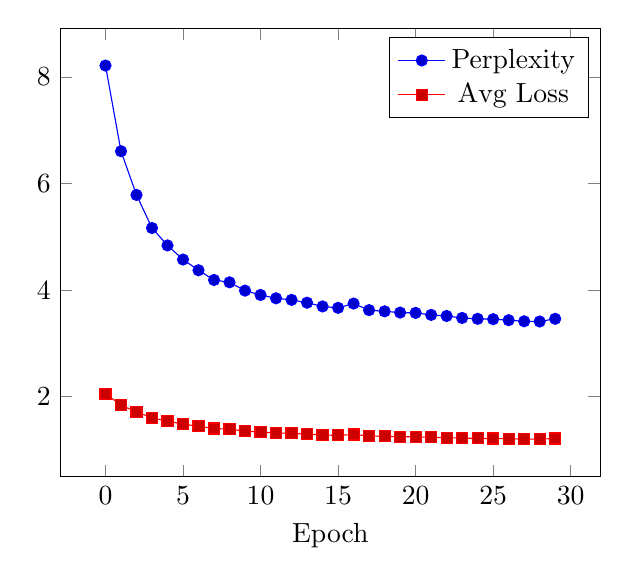
\begin{tikzpicture}
\begin{axis}[
legend entries={Perplexity, Avg Loss},xlabel={Epoch}
]
\addplot coordinates{
(0,8.21193) 
(1,6.60551) 
(2,5.78514) 
(3,5.16428) 
(4,4.83824) 
(5,4.57345) 
(6,4.37238) 
(7,4.18988) 
(8,4.14617) 
(9,3.98995) 
(10,3.90903) 
(11,3.84611) 
(12,3.81673) 
(13,3.76335) 
(14,3.69345) 
(15,3.66706) 
(16,3.74738) 
(17,3.62446) 
(18,3.60159) 
(19,3.57836) 
(20,3.57216) 
(21,3.53473) 
(22,3.51448) 
(23,3.47757) 
(24,3.46120) 
(25,3.45424) 
(26,3.43532) 
(27,3.41468) 
(28,3.41069) 
(29,3.46132) 
};
\addplot coordinates{
(0,2.05614) 
(1,1.84252) 
(2,1.71358) 
(3,1.60438) 
(4,1.54064) 
(5,1.48681) 
(6,1.44391) 
(7,1.40385) 
(8,1.38974) 
(9,1.35636) 
(10,1.33643) 
(11,1.31963) 
(12,1.31209) 
(13,1.29808) 
(14,1.28230) 
(15,1.27432) 
(16,1.29116) 
(17,1.26378) 
(18,1.25551) 
(19,1.24983) 
(20,1.24730) 
(21,1.23787) 
(22,1.23223) 
(23,1.22279) 
(24,1.21800) 
(25,1.21556) 
(26,1.21074) 
(27,1.20495) 
(28,1.20308) 
(29,1.21604) 
};
\end{axis}
\end{tikzpicture}
\caption{Perplexity and Loss with each Epoch}
\label{fig:res}
\end{figure}

In some experiments I encounter exponential overflow / underflow error, so I
change the the data type declared in edf.py from float32 to float64 to avoid
this problem.

\subsection*{Discussion}

The best result of average loss appears at epoch 27, which gives an average loss
of 1.20308. However, the predicted sentence doesn't quite make sense. It is
\begin{tcolorbox}
the agreements bring in the new york stock exchange composite trading the
company 's company 's company 's company 's company 's company 's company 's
company 's company 's company 's company 's company 's company 's company 's
company 's company 's company 's company 's company 's company 's company 's
company 's company 's company 's company 's company 's company 's company 's
company 's company
\end{tcolorbox}
In epoch 29, I get a sentence that makes more sense
\begin{tcolorbox}
the agreements bring is n't disclosed\}
\end{tcolorbox}
However it gives a slightly higher average loss of 1.21604.
\end{document}
